
\section{Computing the First Eigenvalue and Eigenvector of ATA} \label{sec:firstEigen}
Having described the mathematical foundation for ISVD, we will now explore its programmatic implementation. First, we need a method to find an eigenvalue from a matrix. To find the first eigenvector, and in turn the first eigenvalue of the depth matrix $\mtrA$, we can use the following algorithm:
\begin{center}
\begin{enumerate}
    \item Guess a random unit vector with size corresponding to $\mtrA$ (in the case of the Mariana Trench $1440$).
    \item Multiply $\mtrA^T\mtrA$ by the guess vector and divide the result by its magnitude to define the next unit vector.
    \item Use the newly defined unit vector as the updated guess.
    \item Repeat steps $3$ and $4$ until the vector stops changing, this is the first eigenvector $\mvec{V}_1$.
\end{enumerate}
\end{center}
Defined more mathematically, this algorithm is represented as:
\begin{enumerate}
    \item $\mvec{u}_1 = $  a random unit vector with the correct number of components.
    \item $\mvec{u}_{n+1} := \frac{\mtrA^T\mtrA\mvec{u}_{n}}{\lVert \mtrA^T\mtrA\mvec{u}_{n} \rVert}$
    \item Repeat using $\mvec{u}_{n+1}$ as the guess until $\lVert \mvec{u}_{n+1} -  \mvec{u}_{n} \rVert < \text{acceptable precision}$
\end{enumerate}
Note that $\lVert \mvec{u} \rVert$ is the magnitude of the vector $\mvec{u}$ that has $N$ components. Thus, it is defined as:
\begin{align*}
    \lVert\mvec{u}\rVert=\sqrt{\sum \:\:_{i=1}^Nu_i^2}
\end{align*}

Further exploration of why this algorithm works is necessary in a future project. However, a hypothesis as to why this algorithm works could be that we know that the vector ${\mvec{u}_{n}}$ can be expressed using the basis of the eigenvectors from $\mtrA^T\mtrA$, meaning that:
\begin{align*}
    \mtrA^T\mtrA{\mvec{u}_{n}} &= {\mvec{u}_{n}}(\lambda_1\mvec{V_1}\mvec{V_1}^T+\lambda_2\mvec{V_2}\mvec{V_2}^T+...+\lambda_n\mvec{V_n}\mvec{V_n}^T) \\
    &= {\mvec{u}_{n}\lambda_1}(\mvec{V_1}\mvec{V_1}^T+\frac{\lambda_2}{\lambda_1}\mvec{V_2}\mvec{V_2}^T+...+\frac{\lambda_n}{\lambda_1}\mvec{V_n}\mvec{V_n}^T)  \tag{factoring out $\lambda_1$}
\end{align*}
Note that since we are computing the largest eigenvalue, we are assuming that $\lambda_1 >> \lambda_{2...n}$. Then, we normalize the vector so that it has magnitude 1, and perform the multiplication. We repeat this over, and over, lets say we repeat it $g$ times. Then, we can say that:
\begin{align*}
    \mtrA^T\mtrA{\mvec{u}_{n}} 
    &= {\mvec{u}_{n}\lambda_1^g}(\mvec{V_1}\mvec{V_1}^T+(\frac{\lambda_2}{\lambda_1})^g\mvec{V_2}\mvec{V_2}^T+...+(\frac{\lambda_n}{\lambda_1})^g\mvec{V_n}\mvec{V_n}^T) \\  
    &= {\mvec{u}_{n}\lambda_1^g}\mvec{V_1}\mvec{V_1}^T \tag{assuming that $\lambda_1 >> $ all other eigenvalues}\\
    &= {\lambda_1^g}\mvec{V_1}\mvec{V_1}^T  \tag{$\mvec{u}$ is a unit vector, so it is negligible}\\
    &= {\lambda_1^g}
\end{align*}
In other words, as we continue to perform the multiplication and normalization, the eigenvalue ratios go closer and closer to 0, since we are under the assumption that the first eigenvalue is the largest. Then, after enough multiplications, we can estimate those ratios to be zero, leaving a term that can be manipulated to provide the eigenvalue.

Having thus described the algorithm for finding the largest eigenvalue, we can now implement it on our data. Using this algorithm in Matlab (See Section \ref{sec:codeWithOutput}), we find that for the depth matrix $\mtrA$, the first eigenvector, denoted $\mvec{V}_1$, has an eigenvalue of $3.8802*10^{13}$. In addition, we can inspect the components by looking at the plot of $\mvec{V}_1$ as show in \autoref{fig:firstEVect}.
\begin{figure}[H]
    \centering
    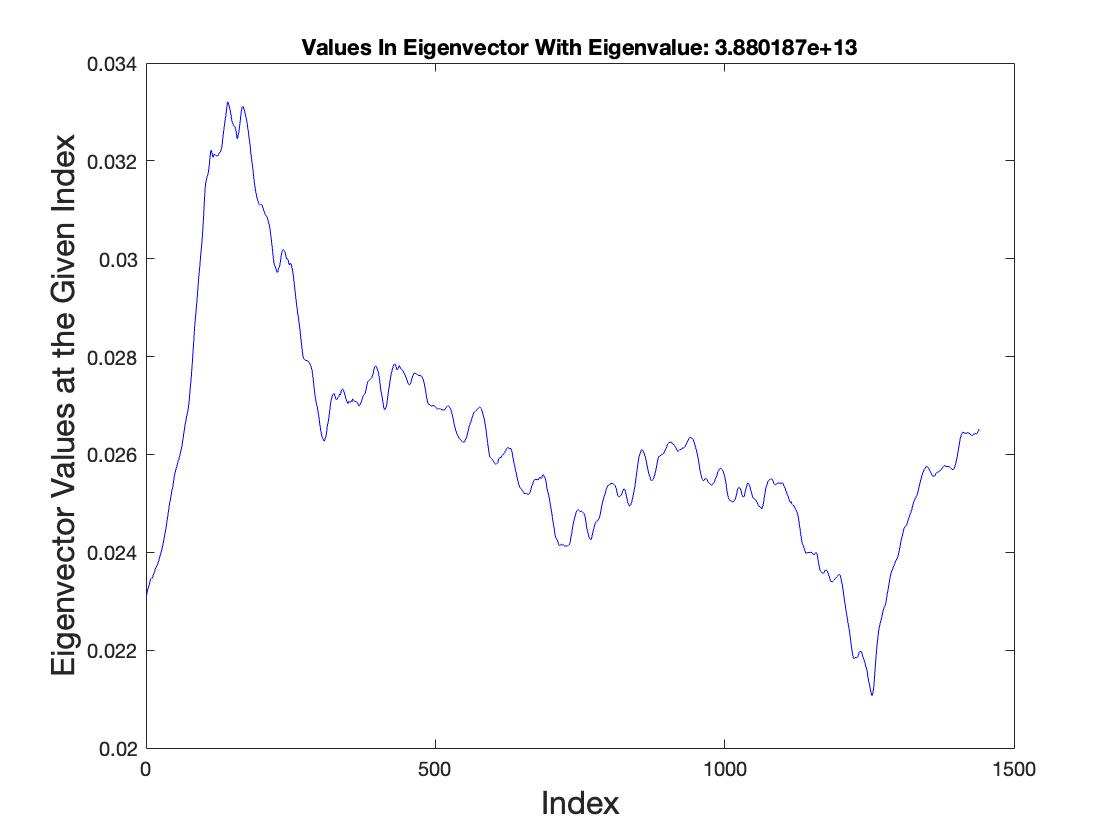
\includegraphics[width=0.6\textwidth]{./imgs/eVect1.jpg}
    \caption{Plot of the Components of $\mvec{V}_1$}
    \label{fig:firstEVect}
\end{figure}